\section{Method}
\label{sec:method}

\subsection{Preliminaries: Native Concept Grounding}

Given an RGB image $X$ and a set of class concepts $\mathcal C$, open-vocabulary semantic segmentation assigns each evaluated pixel a class in $\mathcal C$, with background determined by the benchmark protocol. For class $c$ and its text concept $t_c$, SegEarth-OV3 uses SAM3 to form a condition-dependent state \cite{R10,R11}:
\begin{equation}
H_c=\Phi(X,t_c).
\label{eq:state}
\end{equation}
The state supports three native readouts: a class-level Presence score $p_c$, a dense Semantic map $S_c(x)$, and an Instance map assembled from object-query masks. For query $q$, let $M_{cq}(x)$ be its mask value at pixel $x$ and $r_{cq}$ its raw object confidence. Let $\eta$ be the query-admission threshold and $a_c$ the admission score. The native implementation uses $a_c=p_c$; an anchor-admission variant described below uses the anchor Presence instead. The admitted queries and instance map are
\begin{equation}
\begin{aligned}
Q_c&=\{q:a_c r_{cq}>\eta\},\\
I_c(x)&=\max_{q\in Q_c}M_{cq}(x)r_{cq}p_c.
\end{aligned}
\label{eq:instance}
\end{equation}
Semantic and instance evidence are combined by the native chain
\begin{equation}
F_c(x)=p_c\max\bigl(S_c(x),I_c(x)\bigr).
\label{eq:native-fusion}
\end{equation}
Presence therefore acts on query admission, instance amplitude, and final class scaling. The class maps are compared by pixel-wise argmax, and the baseline threshold assigns low-confidence pixels to background. For a class with aliases, the official path aggregates the prompt-wise outputs in its original order. We denote the resulting single-observation class-score map by $G^{\mathrm{o}}$.

\begin{figure*}[!t]
\centering
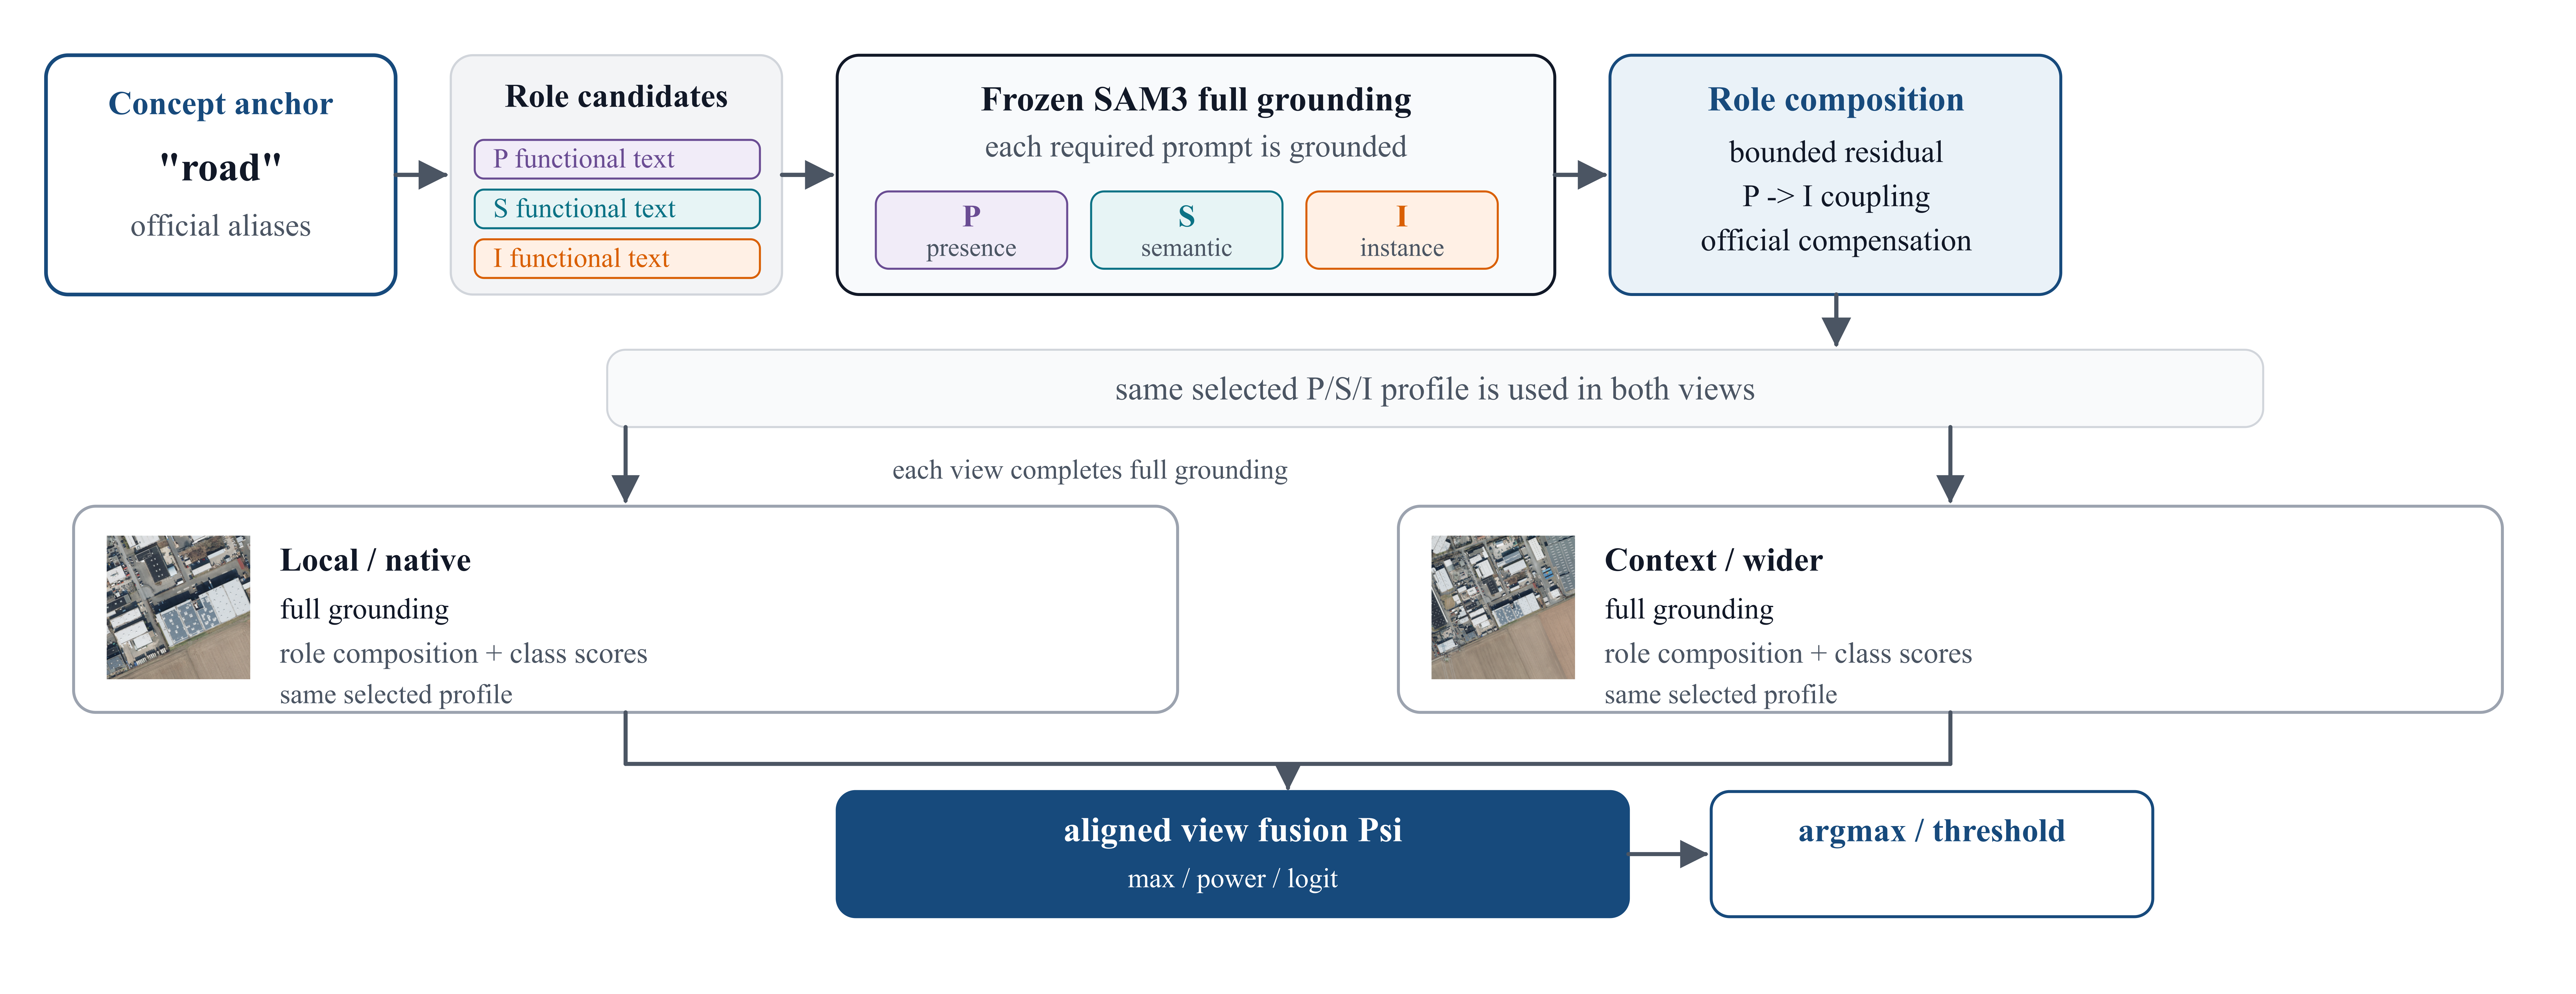
\includegraphics[width=\linewidth]{fig/method_overview.png}
\caption{Overview of Joint Role--View Specialization. Each required prompt is fully grounded by the frozen model. The same selected role profile is applied in Local and Context observations, and complete class-score fields are fused before the original class decision.}
\label{fig:method-overview}
\end{figure*}

 Figure~\ref{fig:method-overview} summarizes the complete evidence path.

\subsection{Role-Functional Text}

The official class name and aliases define an ontology anchor. We keep their native outputs as $(p_c^A,S_c^A,I_c^A)$ and build a small, frozen candidate bank for each class. Presence candidates describe how the concept is established or visible in a scene; Semantic candidates describe dense appearance, surface, coverage, and continuity; Instance candidates describe the organization and separation of query-supported regions. A zero slot keeps the anchor for that role, so not every class requires a non-anchor phrase.

Each non-anchor candidate is grounded through the complete frozen SAM3 model, producing $(p_c^r,S_c^r,I_c^r)$ for $r\in\{P,S,I\}$. We do not route a candidate directly into an isolated head. The assigned readout is combined with its anchor through a bounded residual. For two scalar or spatial quantities $a$ and $b$, define
\begin{equation}
\mathcal B(a,b)=\operatorname{clip}_{[0,1]}\!\left(a+\alpha\,\operatorname{clip}(b-a,-\tau,\tau)\right),
\label{eq:bounded}
\end{equation}
with $\alpha=0.5$ and $\tau=0.25$ in the reported configuration. The Presence and Semantic updates are
\begin{equation}
\begin{aligned}
\tilde p_c&=\mathcal B(p_c^A,p_c^{\pi_P}),\\
\tilde S_c(x)&=\mathcal B(S_c^A(x),S_c^{\pi_S}(x)).
\end{aligned}
\label{eq:role-updates}
\end{equation}
Because Presence affects instance construction, the instance maps are rebuilt after the Presence update. With admission score $a$, the anchor and candidate instance maps are
\begin{equation}
\begin{aligned}
I_A^{\tilde p}&=\mathcal I(Q_A;\tilde p,a),\\
I_{\pi_I}^{\tilde p}&=\mathcal I(Q_{\pi_I};\tilde p,a),\\
\tilde I_c&=\mathcal B(I_A^{\tilde p},I_{\pi_I}^{\tilde p}),
\end{aligned}
\label{eq:instance-rebuild}
\end{equation}
where $\mathcal I$ denotes the query aggregation in Eq.~\eqref{eq:instance}. The role-composed class evidence is then
\begin{equation}
F_{\pi,c}(x)=\tilde p_c\max\bigl(\tilde S_c(x),\tilde I_c(x)\bigr).
\label{eq:role-final}
\end{equation}
For native admission, $a=\tilde p_c$; for anchor admission, only query membership uses $a=p_c^A$, while the amplitude and final scaling still use the updated Presence. If all role slots are zero, the updates reduce to the anchor.

The official score field is retained to preserve aliases and the baseline aggregation order. Let $G_v^{\mathrm{o}}$ be the official map for observation $v$, $F_{v,\pi}$ the role-composed map, and $F_v^A$ the anchor composition without supplementary text. The observation-level output is
\begin{equation}
G_{v,\pi}=\operatorname{clip}_{[0,1]}\!\left(G_v^{\mathrm{o}}+F_{v,\pi}-F_v^A\right).
\label{eq:official-compensation}
\end{equation}
Thus, disabling all role updates returns the official map exactly. The construction is not an ensemble of three independent predictions: candidates are re-grounded completely, only their assigned readout changes the anchor, and the native Presence--Instance coupling remains active.

\subsection{Aligned Local and Context Observations}

A text description can specify a continuous surface or a complete region, but it cannot create visual evidence absent from the observation. Local observations preserve effective sampling density for boundaries and small objects; Context observations expose a wider spatial layout and long-range continuity. For datasets supplied as coordinate tiles, Context observations are assembled from spatially aligned neighboring RGB tiles without neighboring labels; otherwise they are enlarged crops of the input image. The evaluation protocol specifies the exact construction.

Every observation completes the native grounding and role composition independently. The Local and Context observations reuse the same selected role profile; JRV does not assign Presence to one view, Semantic to a second, or Instance to a third. For a view family $v\in\{L,G\}$ with target units $\mathcal U_v$, each unit $u$ produces a role-composed map $G_{u,\pi}$ on its own coordinate system. Let $W_u$ restore the map to the target coordinates and let $w_u(x)$ indicate valid coverage. The aligned view evidence is
\begin{equation}
\overline G_{v,c}(x)=
\frac{\sum_{u\in\mathcal U_v}w_u(x)\,W_u[G_{u,\pi,c}](x)}
{\sum_{u\in\mathcal U_v}w_u(x)}.
\label{eq:view-average}
\end{equation}
The final class-score field is
\begin{equation}
\begin{aligned}
Z_c(x)&=\Psi_{\omega}\!\left(\overline G_{L,c}(x),\overline G_{G,c}(x)\right),\\
\widehat Y&=\mathcal D_{\mathrm{base}}(Z),
\end{aligned}
\label{eq:view-fusion}
\end{equation}
where $\mathcal D_{\mathrm{base}}$ retains the baseline argmax and background threshold. The profile operator $\Psi_{\omega}$ is fixed rather than learned. We use element-wise maximum, Local or Context endpoints, weighted power means, and weighted logit fusion:
\begin{equation}
\begin{aligned}
\Psi_{\max}(L,G)&=\max(L,G),\\
\Psi_{\rho,g}(L,G)&=\left((1-g)L^{\rho}+gG^{\rho}\right)^{1/\rho}.
\end{aligned}
\label{eq:view-operators}
\end{equation}
The logit variant uses the same mixture in log-odds space:
\begin{equation}
\Psi_{\mathrm{logit},g}(L,G)=\sigma\!\left((1-g)\operatorname{logit}(L)+g\operatorname{logit}(G)\right).
\label{eq:logit-operator}
\end{equation}
The operator family is a profile choice, not a new learned attention module. Combining complete class-score fields preserves the native cross-category decision after role and view composition.

\begin{figure*}[!t]
\centering
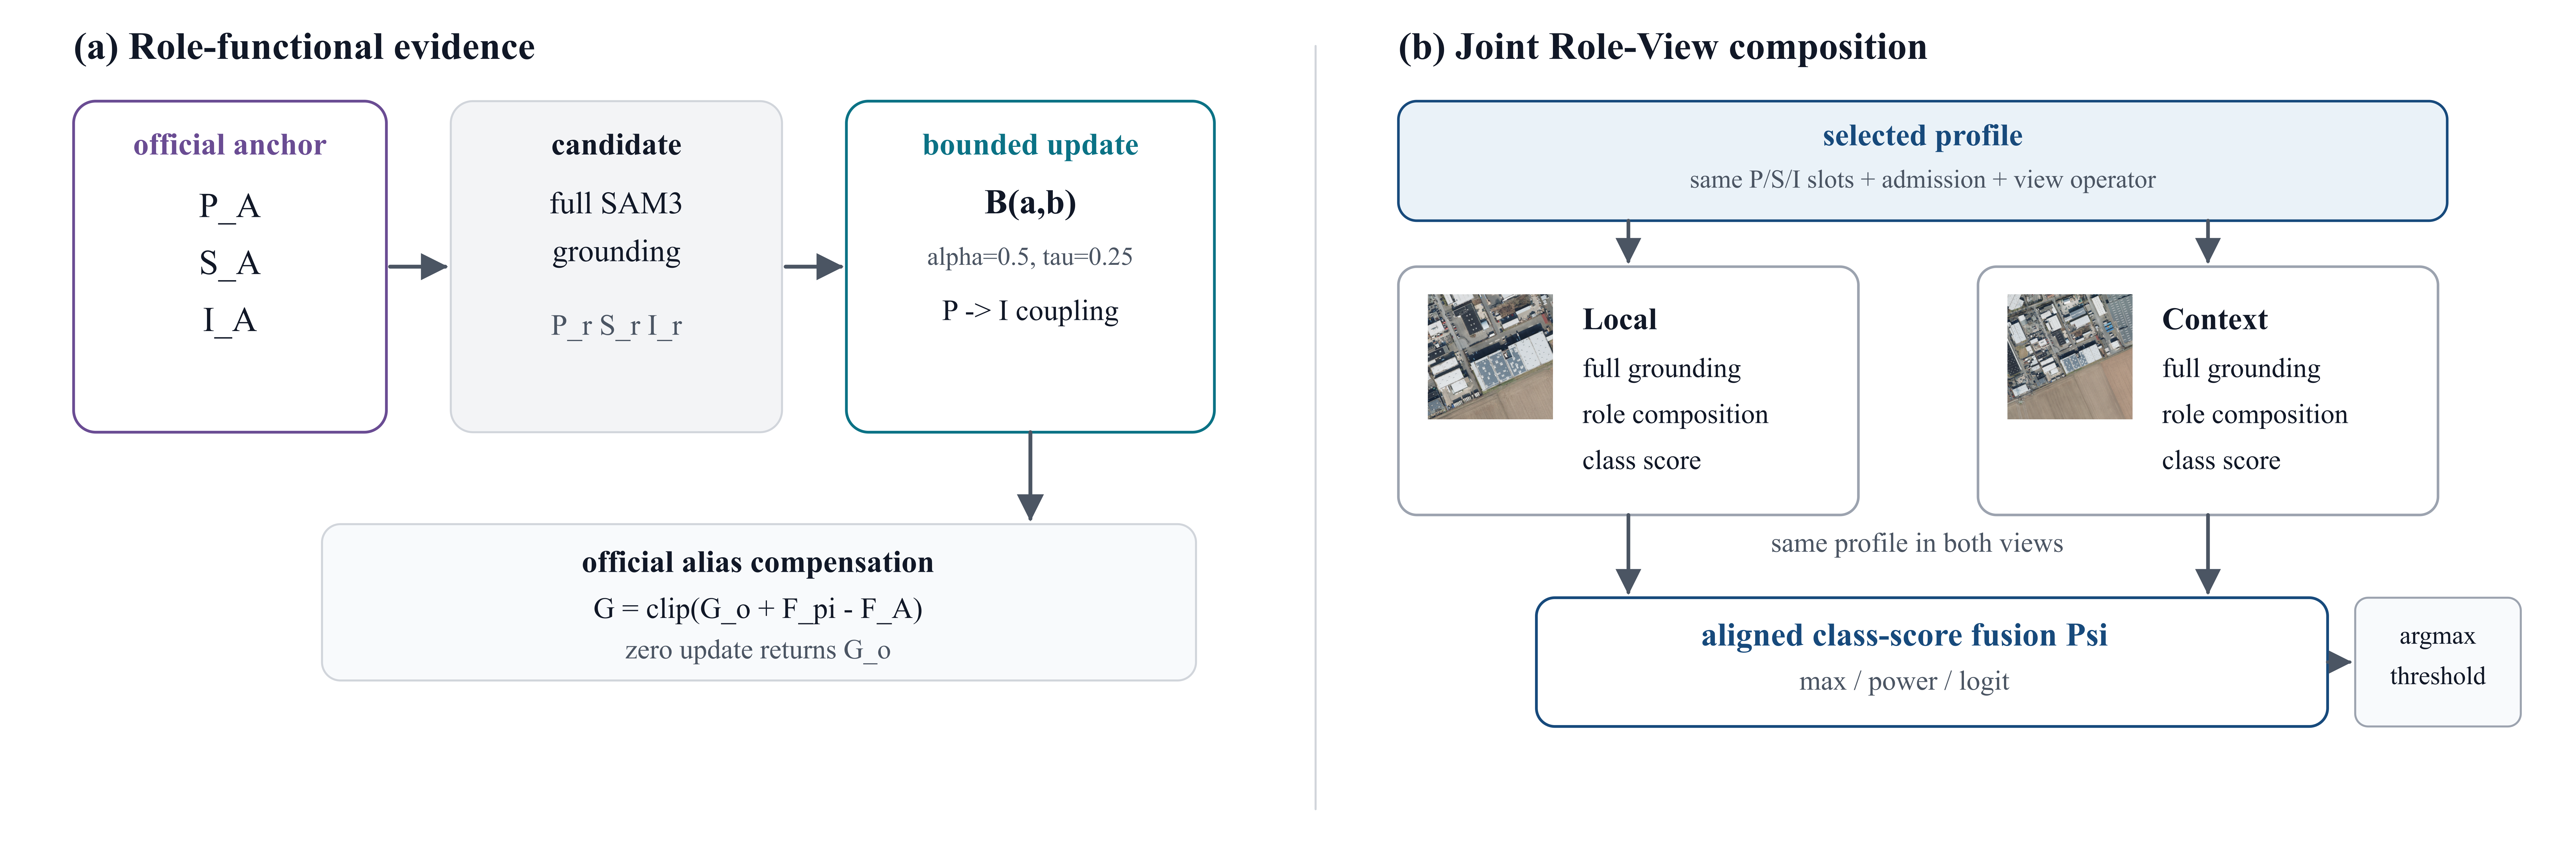
\includegraphics[width=\linewidth]{fig/method_detail.png}
\caption{Method details. (a) Role-functional evidence keeps the official anchor, applies bounded role updates, rebuilds Instance after the Presence update, and restores the official map through alias compensation. (b) Local and Context observations reuse the same profile and are fused after complete class-score composition.}
\label{fig:method-detail}
\end{figure*}

 Figure~\ref{fig:method-detail} isolates the two evidence interactions.

\subsection{Inference Protocol and Profile Definition}

A dataset profile is a fixed tuple
\begin{equation}
\pi=(s_P,s_S,s_I,a,\Psi_{\omega}),
\label{eq:profile}
\end{equation}
where each $s_r$ indexes a candidate slot in the frozen text bank, $s_r=0$ retains the anchor, $a$ specifies native or anchor admission, and $\Psi_{\omega}$ specifies the view operator. The same profile is applied to every image in a benchmark and to both Local and Context observations. The text bank and profile are fixed before inference; SAM3 weights are never updated. Profile selection is dataset-level and offline, and the experimental section reports the selection protocol. No image-level ground-truth routing is used.

Three implementation properties connect the method to the experimental analysis. Every required supplementary phrase undergoes full native grounding rather than modifying an isolated decoder state. An unchanged slot or an all-zero role profile recovers the anchor path, including the official alias aggregation. Local and Context outputs are combined only after complete role composition and coordinate restoration, so the method changes evidence use rather than SAM3 attention or its internal fusion operator.

